% === R029 Fig. 1: Protocol-Centered Hero ===
\begin{figure*}[t]
    \centering
    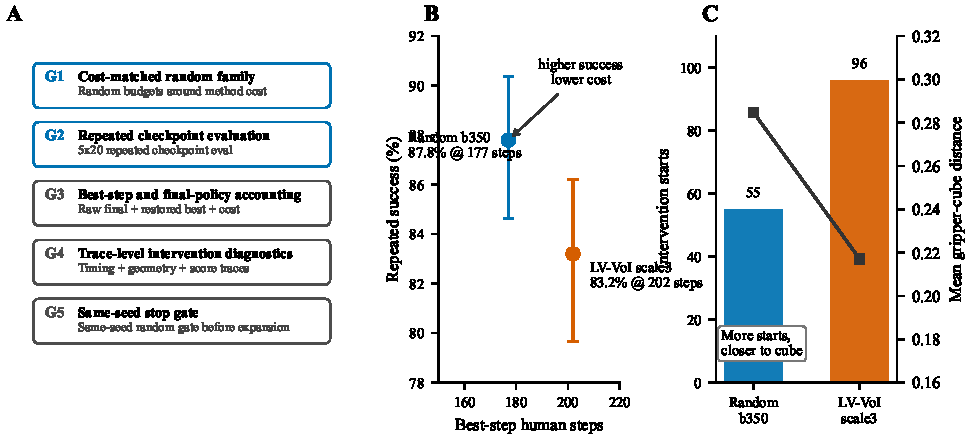
\includegraphics[width=0.95\textwidth]{figures/fig1_protocol_hero_r029.pdf}
    \caption{Diagnostic protocol for HIL-RL intervention-trigger claims. The protocol requires cost-matched random families, repeated checkpoint evaluation, best/final policy accounting, trace-level intervention diagnostics, and a same-seed stop gate before expansion. Applied to robosuite Lift, it reverses an initially plausible LV-VoI conclusion: \texttt{random\_b350} achieves higher repeated success at lower best-step human cost than LV-VoI scale3. Trace diagnostics show that LV-VoI starts more interventions while starting closer to the cube, rejecting a simple far-from-object explanation.}
    \label{fig:protocol_hero}
\end{figure*}

% === R029 Table: Protocol Checklist ===
\begin{table*}[t]
\centering
\caption{Diagnostic protocol checklist for HIL-RL intervention-trigger claims. Each gate is motivated by a failure mode surfaced in the Lift/Stack case study.}
\label{tab:protocol_checklist}
\begin{tabular}{p{0.07\textwidth}p{0.19\textwidth}p{0.32\textwidth}p{0.33\textwidth}}
\toprule
Gate & Requirement & What to report & Why it matters \\
\midrule
G1 & Cost-matched random family & At least one random budget below and above the method's realized human cost; report realized best-step human cost, not only nominal budget. & Prevents a learned trigger from appearing efficient only because the random baseline was mismatched. \\
G2 & Repeated checkpoint evaluation & Evaluate selected checkpoints with repeated episodes; report binomial confidence intervals and seed variability. & Single restored or final evaluations can change rankings in noisy RL settings. \\
G3 & Best-step and final-policy accounting & Report raw final policy, restored best policy, and best-step human cost. & Separates late collapse/checkpoint selection from true intervention efficiency. \\
G4 & Trace-level intervention diagnostics & Log intervention starts with timing, budget fraction, task geometry, score, and p\_fail when available. & Explains how a trigger spends budget and tests mechanism hypotheses. \\
G5 & Same-seed stop gate & Before expanding a repaired trigger, compare it against same-seed cost-matched random using repeated evaluation. & Stops weak heuristic repairs before expensive expansion and prevents over-tuning. \\
\bottomrule
\end{tabular}
\end{table*}

